% !TeX encoding = UTF-8
\section{Einleitung}
Der Traum vom autonomen Fahren reicht bis in die Antike zu den Griechen zurück, deren Gott des Feuers und der Schmiedekunst Hephaistos Androiden und selbst fahrende Automobile konstruierte. Mittlerweile ist die Forschung in diesen Bereichen von der Phantasie in die Wirklichkeit gerückt und so weit fortgeschritten, dass dieser Traum schon bald Wirklichkeit werden könnte. Zuvor müssen jedoch etliche Herausforderungen bewältigt werden. Eine davon ist, das Auto sicher durch den Straßenverkehr zu bringen. Dabei heißt sicher, dass das Auto während der Fahrt weder sich noch andere Verkehrsteilnehmer gefährdet. Neben der Sicherheit ist jedoch auch das möglichst schnelle Erreichen des Ziels wichtig, bei dem das Auto seinen Weg durch eine Umgebung mit statischen und dynamischen, das heißt sich bewegenden Hindernissen finden muss. In diesem Kontext ist noch zu erwähnen, dass dieser Weg nicht wie bei einem Navigationssystem beispielsweise von Berlin nach Hamburg führt, sondern eher von einer Straßenecke zur nächsten oder über einen Parkplatz. Dies wird durch einen Pfadplaner gewährleistet, der -informell gesprochen - aus der eigenen Position, dem Zielbereich und unter Berücksichtigung aller statischen und sich bewegenden Hindernissen einen sicheren Pfad zum Ziel findet. Dieser Pfad ist dann durch das Auto abfahrbar.\\
Um diese Aufgabe zu meistern, existieren unterschiedliche Ansätze, um dem Auto je nach Anwendungsfall bei gegebenen Ziel eine \textit{Trajektorie} vorzuschlagen. Die jeweiligen Algorithmen unterscheiden sich in Ausführungszeit, Genauigkeit, Sicherheit und berechnen unterschiedlich optimale Pfade.  \\
Das Dahlem Center for Machine Learning and Robotics untersucht maschinelles Lernen und Anwendungen intelligenter Systeme. Dazu haben sich vier Arbeitsgruppen der Freien Universität Berlin zusammengeschlossen:
\begin{itemize}
\item Intelligent Systems and Robotics (Prof. Dr. Raúl Rojas)
\item Autonomos Cars (Prof. Dr. Daniel Göhring)
\item Artifical and Collective Intelligence (Prof. Dr. Tim Landgraf)
\item Logic and automatic proofs (Christoph Benzmüller)
\end{itemize}
Ein Forschungsgebiet ist die Entwicklung und Analyse autonomer Autos. Zur oben beschriebenen Pfadplanung wird in der Arbeitsgruppe hauptsächlich das Prinzip elastischer Bänder (Time-Elastic-Bands, \citep[vgl.][]{RoeHoBe}) zur Erzeugung abfahrbarer \textit{Trajektorien} benutzt. Doch auch die Untersuchung und Analyse anderer Algorithmen ist interessant, um zu überprüfen, ob sich eine vertiefte Forschung in diesen Bereichen lohnt. \\ 
Diese Bachelorarbeit untersucht einen dieser anderen Algorithmen zur Pfadplanung, \textit{RRT*}, auf seine Tauglichkeit, über eine vorgegebene Fahrbahn mit Hindernissen eine abfahrbare, sichere und möglichst optimale \textit{Trajektorie} zu finden. 

\subsection{Aufbau und Struktur}
Nach einer kurzen Hinführung zum Thema werden zuallererst die Grundlagen (\ref{sec:Grundlagen}) besprochen, um das Verständnis der nachfolgenden Kapitel zu erleichtern. Danach wird die Umsetzung des Algorithmus auf das Auto sowie die technischen Details und Hintergründe beschrieben (\ref{sec:Umsetzung}). Im vierten Kapitel (\ref{sec:Ergebnisse}) werden die Ergebnisse der Testfahrten vorgestellt und bewertet. Zum Schluss (\ref{sec:Zusammenfassung}) werden in einem Fazit alle Schlussfolgerungen nochmals zusammengefasst und ein Ausblick auf weitere mögliche Forschungsmöglichkeiten gegeben. \\ 
\subsubsection{Problemanalyse}
\label{sec:Problemanalyse}
Diese Arbeit untersucht die Effizienz des\textit{ RRT*}-Algorithmus unter Anwendung bei autonomen Autos. Dazu fährt das Auto eine vorgegebene Strecke ab.
\begin{figure}
\centering
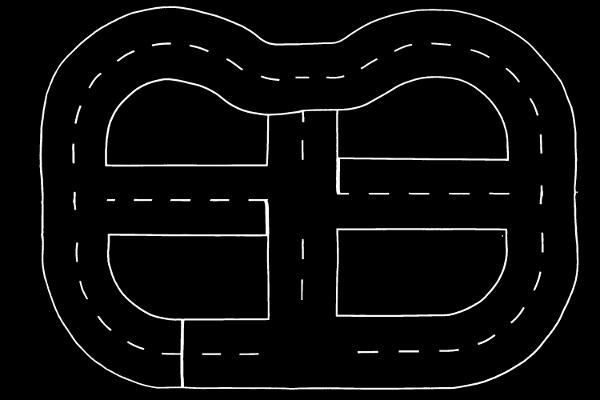
\includegraphics[scale=0.5]{Bilder/fu_robotics_lab_map_600x400.png} 
\caption{Das Auto fährt auf der äußeren Strecke einmal im Kreis}
\end{figure}
 Auf dieser Strecke werden erst statische, dann sich bewegende Hindernisse platziert. \\
Das Auto soll diese Strecke in möglichst kurzer Zeit mit einem möglichst optimalen Pfad abfahren, ohne eines dieser Hindernisse zu berühren. Dazu sollte das Auto den Algorithmus idealerweise 30 Mal pro Sekunde ausführen, mindestens aber vier Mal pro Sekunde. Dadurch wird gewährleistet, dass der entstehende Pfad fürs Auto sich an bewegende Hindernisse anpasst. \\
Die Effizienz, Sicherheit und Effektivität des Algorithmus wird bei verschiedenen Eingabeparametern untersucht und bewertet. \\

\subsubsection{Anmerkung zur Gestaltung der Arbeit}
[TODO Plagiat mit Prof abklären (ist ne 1:1 Kopie)]
Für die im Folgenden verwendeten personenbezogenen
Ausdrücke wurde, um die Lesbarkeit der Arbeit zu erhöhen,
ausschließlich die männliche Schreibweise gewählt. Desweiteren werden eine
Reihe von englischen Bezeichnungen und Fachwörtern verwendet, um einerseits dem
interessierten Leser das Studium der fast ausschließlich englischen
Fachliteratur zu erleichtern und andererseits bestehende Fachbegriffe nicht durch die Übersetzung zu verfälschen. Bei diesen Begriffen wird zur Unterscheidung eine kursive Schriftart verwendet.
[TODO: Wenn möglich, wurden die Quellen angegeben, bei den anderen wurde zur Definition Wikipedia verwendet.]

\subsubsection{Glossar}
\begin{tabularx}{\textwidth}{l|X}
 \textbf{Begriff}  & \textbf{Erklärung}  \\
\hline Trajektorie & Die Strecke, die dem Low-Level-Planer des Autos übergeben wird\\
Low-Level-Planer & Steuert direkt die Motoren des Autos, Lenkung und Antrieb, um eine vorgegebene Trajektorie möglichst genau abzufahren. \\
RRT & Rapidly-Exploring Random Tree \citep{Lav98}, ein Algorithmus zur Findung eines Pfades zum Ziel durch unbekanntes Gelände, wird in Kapitel \ref{RRT} noch weiter erläutert\\
RRT* & Eine verbesserte Variante des RRT, bei dem die Pfade optimiert werden \citep{KaFra10}. Asymptoptisch optimal, erläutert in Kapitel \ref{RRT*} \\
ROS & Robot Operating Systems, eine Open-Source Sammlung an Software-Bibliotheken und Werkzeugen zur Kreation von Anwendungen zur Robotik \citep{ROS}. \\
Nonholonomic Robots & Roboter, die gewissen kinematischen Einschränkungen unterworfen sind. Ein Auto zum Beispiel kann sich nicht in jede beliebige Richtung bewegen, sondern ist z.B. durch den maximalen Lenkwinkel und den Wenderadius eingeschränkt und kann nicht jeden beliebigen Punkt sofort, mit nur einem Schritt, erreichen. Im Gegensatz dazu stehen holonome Roboter, die sich in jede beliebige Richtung ohne direkte Einschränkungen bewegen können.  \\
Kinodynamic planning & Beschreibt eine Klasse von Problemen, bei der physikalische Einschränkungen wie Geschwindigkeit, Beschleunigung und Kräfte zusammen mit kinematischen Einschränkungen (z.B. Hindernisvermeidung) berücksichtigt werden müssen. \\
hochdimensionale Probleme & Probleme, bei deren Lösung nicht nur ein oder zwei, sondern sehr viele verschiedene Parameter berücksichtig werden müssen. Kinodynamic Planning befasst sich mit hochdimensionalen Problemen.\\
randomisierte Algorithmen & Algorithmen, deren Durchführung nicht determiniert ist, die also jedesmal ein etwas anderes Ergebnis zurückliefern. Der Vorteil ist, dass dies Algorithmen zwar nicht immer das bestmöglichste Ergebnis liefern, dafür aber schneller in der Ausführungszeit sind und oft einfacher zu verstehen und zu implementieren.\\
\end{tabularx} 

\begin{tabularx}{\textwidth}{l|X}
 \textbf{Begriff}  & \textbf{Erklärung}  \\
\hline 
Odroid & Einplatinencomputer am Auto mit Mehrkernprozessor. \\
Arduino Nano & Mikrocontroller am Auto zur Steuerung der Motoren und Sensoren.\\
Gyroskop & Auch Kreiselinstrument, Sensor am Auto zur Messung der Lageänderung (z.B. Ausrichtung des Autos).\\
Lidar & Light detection and ranging; Radarscanner am Auto, für Abstandsmessung zu Hindernissen.\\
Odometrie & Methode zur Schätzung von Position und Orientierung anhand der Daten des Vortriebsystems (Motoren).\\
Rewiring & Neuverknüpfung eines RRT*-Baumes \citep{KaFra10}. Die Begriffe Rewiring und Neuverknüpfung werden synomym gebraucht. Nach Hinzufügung eines Knotens K zum Baum werden Nachbarknoten überprüft, ob diese durch K besser erreichbar sind als vorher. Falls ja, wird K als Vaterknoten ausgewählt. \\
k-nearest neighbour algorithm & Algorithmus, der zu einem Punkt P die nächsten K Nachbarn bestimmt.\\
radius k-nearest neighbour & Algorithmus, der in einem Radius alle nächsten Nachbarn des Punktes P bestimmt.\\
Quaternion & 4-dimensionaler Vektor, in dem die Ausrichtung eines Objekts im Raum definiert ist.\\
\end{tabularx}
\subsubsection{Wichtige Quellen und deren Beitrag zum Thema}
Als wichtigste Quellen sind "Rapidly Exploring Random Trees: A new Tool for Path Planning"\citep{Lav98} von Steven LaValle und "Incremental Sampling-based Algorithms for Optimal Motion Planning" \citep{KaFra10} von Sertac Karaman und Emilio Frazzoli zu nennen. Diese führen jeweils die Algorithmen RRT und RRT* ein. Eine besonders am Anfang sehr wichtige Quelle war "Optimal Path Planning using RRT* based Approaches: A Survey and Future Directions"\citep{NoKhaHa16}, welche eine Übersicht über verschiedene Variationen und RRT* in verschiedenen Szenarien gibt. Dies hat mir bei der Orientierung und Eingrenzung des Themas sehr geholfen. [TODO Kapitel erscheint irgendwie sinnlos...kann man da iwie sinn hinzufügen?]\\
Nun werden wir uns den wissenschaftlichen Grundlagen der Arbeit widmen.

